% !TeX program = xelatex
% 这是编辑模板；build_report.py会展开表格至report_ready.tex，再用XeLaTeX编译后者两次。
\documentclass[UTF8,zihao=-4,fontset=fandol]{ctexart}
\usepackage[a4paper,left=22mm,right=20mm,top=23mm,bottom=21mm,headheight=15pt]{geometry}
\usepackage{fontspec,amsmath,amssymb,graphicx,booktabs,array,tabularx,longtable}
\usepackage[table]{xcolor}
\usepackage{float,caption,fancyhdr,enumitem,hyperref,attachfile2,fvextra}
\IfFileExists{/Users/john/Library/Fonts/NotoSerifCJKsc-Regular.otf}{
\setCJKmainfont[Path=/Users/john/Library/Fonts/,BoldFont=NotoSerifCJKsc-Bold.otf]{NotoSerifCJKsc-Regular.otf}
\setCJKsansfont[Path=/Users/john/Library/Fonts/,BoldFont=NotoSansCJKsc-Bold.otf]{NotoSansCJKsc-Regular.otf}}{}
\setmainfont[BoldFont=texgyretermes-bold.otf,ItalicFont=texgyretermes-italic.otf,BoldItalicFont=texgyretermes-bolditalic.otf]{texgyretermes-regular.otf}
\setmonofont{lmmono10-regular.otf}
\hypersetup{colorlinks=true,linkcolor=black,urlcolor=blue!55!black,
  pdftitle={基于高频量价特征的多因子选股实证分析},pdfauthor={岳瀚阳}}
\definecolor{headerblue}{RGB}{15,47,87}
\definecolor{papergray}{RGB}{245,247,249}
\graphicspath{{figures/}}
\captionsetup{font=small,labelfont=bf,labelsep=quad,skip=5pt}
\setlist{nosep,leftmargin=2em,topsep=4pt}
\renewcommand{\arraystretch}{1.28}
\setlength{\tabcolsep}{5pt}
\setlength{\parindent}{2em}
\setlength{\parskip}{3pt}
\setlength{\emergencystretch}{2em}
\linespread{1.23}
\setcounter{tocdepth}{1}
\ctexset{section={name={,},number=\chinese{section},format=\large\bfseries,
    beforeskip=12pt,afterskip=7pt},subsection={format=\normalsize\bfseries,beforeskip=9pt,afterskip=4pt}}
\pagestyle{fancy}
\fancyhf{}
\fancyhead[L]{\small 岳瀚阳\quad 3230104443}
\fancyhead[R]{\small《量化投资》课程作业}
\fancyfoot[C]{\small\thepage}
\renewcommand{\headrulewidth}{0.4pt}
\newcommand{\ReportDate}{2026年11月14日}
\newcommand{\ReportTitle}{基于高频量价特征的多因子选股实证分析}
\newcommand{\navfigure}[2]{\begin{figure}[H]\centering
  \includegraphics[width=0.97\linewidth,height=0.413\textheight,keepaspectratio]{#1.pdf}
  \caption{#2。上图为五个独立多头组，下图为50\%多头、50\%空头目标的费后理论组合。}
  \end{figure}}
\newcommand{\MaxCorr}{0.330}
\newcommand{\MaxCorrPair}{CDPDP与Amplitude}
\newcommand{\ModelWeekReturn}{4.49\%}
\newcommand{\ModelWeekSharpe}{1.11}
\newcommand{\ModelWeekDD}{-7.25\%}
\newcommand{\ModelWeekIC}{0.041}
\newcommand{\ModelWeekRank}{0.048}
\newcommand{\ModelBiweekReturn}{2.08\%}
\newcommand{\ModelBiweekSharpe}{0.55}
\newcommand{\ModelBiweekDD}{-4.20\%}
\newcommand{\ModelBiweekIC}{0.041}
\newcommand{\ModelBiweekRank}{0.045}
\newcommand{\ModelMonthReturn}{2.94\%}
\newcommand{\ModelMonthSharpe}{0.80}
\newcommand{\ModelMonthDD}{-3.59\%}
\newcommand{\ModelMonthIC}{0.054}
\newcommand{\ModelMonthRank}{0.042}
\newcommand{\CPVMonthReturn}{7.14\%}
\newcommand{\CPVMonthSharpe}{1.79}
\newcommand{\CPVBiweekReturn}{4.73\%}
\newcommand{\ComparisonStart}{2017-02-03}
\newcommand{\ReturnStart}{2017-02-06}
\newcommand{\ComparisonEnd}{2018-12-28}
\newcommand{\ReturnDays}{468}
\newcommand{\CommonRows}{101,815}
\newcommand{\CommonMeanStocks}{217.1}
\newcommand{\ModelsCount}{69}
\newcommand{\AllSeries}{234}
\newcommand{\TradesCount}{1,898,300}
\newcommand{\OOSStaleSeries}{25}
\newcommand{\OOSUnclosedSeries}{50}
\newcommand{\OOSLSStaleCases}{4}
\newcommand{\OOSLSUnclosedCases}{11}

\begin{document}

\begin{titlepage}
\thispagestyle{empty}
\centering
\vspace*{-8mm}

\includegraphics[width=0.65\linewidth]{char.png}\par
\vspace{12mm}

\includegraphics[width=0.43\linewidth]{logo.png}\par
\vspace{9mm}
{\LARGE\bfseries《量化投资》\par}
\vspace{4mm}
{\Large\bfseries\ReportTitle\par}
\vspace{3mm}
{\large 基于XGBoost的滚动合成与日频持仓回测\par}
\vspace{13mm}
\renewcommand{\arraystretch}{1.7}
\begin{tabular}{rl}
姓\quad 名 & \underline{\makebox[68mm]{岳瀚阳}}\\
学\quad 号 & \underline{\makebox[68mm]{3230104443}}\\
学\quad 院 & \underline{\makebox[68mm]{管理学院}}\\
日\quad 期 & \underline{\makebox[68mm]{\ReportDate}}\\
指导老师 & \underline{\makebox[68mm]{曾涛、彭旺}}\\
\end{tabular}
\vfill
{\small 数据区间：2016年至2018年\quad 修订版：统一标签、执行与绩效口径}
\end{titlepage}
\setcounter{page}{2}

\begin{center}
{\Large\bfseries\ReportTitle}\par\vspace{4pt}
{\normalsize 岳瀚阳\quad 3230104443}
\end{center}
\noindent\textbf{摘要}\quad
本文沿用原作业的六个高频量价因子，分别研究SmartMoney、CPV、CDPDP、日内偏度、尾盘收益和振幅，
并采用XGBoost进行非线性合成。首先对2016至2018年动态中证500成分进行完整单因子检验，随后以
\ComparisonStart 至\ComparisonEnd 为共同样本外信号区间，对模型与单因子作公平比较。
标签统一为次日开盘开始的5、10、20交易日连续价格收益；模型每月滚动更新，训练标签须在预测月开始前实现。
每种策略分别记录现金、持仓、实际成交和费用，净值图与风险指标来自同一日收益账本。

样本外结果显示，XGBoost周频、双周频、月频理论多空组合的年化收益分别为
\ModelWeekReturn、\ModelBiweekReturn、\ModelMonthReturn，Sharpe分别为
\ModelWeekSharpe、\ModelBiweekSharpe、\ModelMonthSharpe。
模型具有正向截面排序信息，但没有全面优于单因子；同样本下月频CPV的年化收益为\CPVMonthReturn，
Sharpe为\CPVMonthSharpe。多数多头组仍出现绝对亏损，说明多空收益与多头盈利应分别评价。
结果依赖开盘成交代理、可借券和缺失行情估值假设，不代表可直接实现的实盘收益。

\noindent\textbf{关键词}\quad 高频量价；因子分层；XGBoost；滚动训练；日频持仓回测
\vspace{3mm}
\tableofcontents

\clearpage
\section{课题具体说明}
本课题使用分钟行情提取交易行为与价格分布特征，研究它们对股票未来截面收益排序的解释能力。
研究对象为历史动态中证500成分，采用六因子体系，并通过树模型检验非线性合成是否能够改善选股表现。
实证回答三个问题：单因子的方向是否稳定；预测期限与调仓频率一致后绩效如何；XGBoost在共同测试样本上能否优于单因子。

本次保留原报告的章节框架，但按修正后的程序重新计算全部数据与图像。
原始\texttt{code2.py}为纯因子流程；新增\texttt{code2\_xgboost.py}完成模型合成。
原报告中的XGBoost旧数值没有直接用于本文，全部模型统计来自本次真实滚动训练。
文中只比较已执行的固定参数实验，不将因子解释或回测排序视为市场机制的因果证明。

\section{数据描述与处理}
\subsection{数据来源与样本区间}
数据均来自课程本地资料，未添加外部行情。分钟数据位于
\path{data/bar_1m_2016_2018/}，共731个交易日文件。日行情补入2015年历史作为风格变量预热，
同时使用交易日历、历史指数成分、行业公告与总市值。程序为计算历史读取806只候选股票，
实际信号日是否进入股票池仍由当天成分记录决定。

\begin{table}[H]\centering\small
\caption{主要数据字段及用途}
\begin{tabularx}{\linewidth}{p{28mm}X}
\toprule 数据类别 & 字段与用途\\\midrule
分钟行情 & time、symbol、OHLC、volume、amount；构造六个日内统计量。\\
日行情 & OpenPrice、ClosePrice、PrevClosePrice；建立连续价格、执行价格与每日估值。\\
交易与股本 & PTFlag、TradingVolumes、NonRestrictedShares、AFloats；停牌识别及换手率控制。\\
指数成分 & date、symbol；按日取历史成分，不用最新成分回填。\\
行业与市值 & 公告日期、tag、tot\_cap；行业及对数总市值中性化。\\
交易日历 & TradingDay；定义滚动窗口、标签期限和预定调仓日期。\\\bottomrule
\end{tabularx}\end{table}

完整单因子信号从2016-01-29开始，收益从下一交易日计入，至2018-12-28结束，共711个日收益。
XGBoost首个预测月为2017年2月，共同信号起点为\ComparisonStart，收益起点为\ReturnStart，
共同回测包含\ReturnDays 个日收益。模型输入要求当日六因子均有效，因此共同样本有\CommonRows 条股票日记录，
日均约\CommonMeanStocks 只股票。这个完整输入子样本小于每天约500只成分，结论的适用范围应据此理解。

\clearpage
\subsection{连续价格、信息时点与特征工程}
原始日行情不是可直接跨除权日计算收益的连续价格。令$C^{\rm last}_{i,t-1}$为最后有效实际收盘，
$P^{\rm ref}_{i,t}$为当日除权参考昨收，使用向前累计调整：
\begin{equation}
 a_{i,t}=a_{i,t-1}\frac{C^{\rm last}_{i,t-1}}{P^{\rm ref}_{i,t}},\qquad
 \widetilde O_{i,t}=a_{i,t}O_{i,t},\quad \widetilde C_{i,t}=a_{i,t}C_{i,t}.
\end{equation}
调整仅使用当时及历史信息；已知停牌沿用估值，重新交易时处理累计调整。
若历史中间存在无法解释的行情缺口，程序停止并要求补全数据，避免把漏记涨跌当作除权。
例如603528在2017-06-07的原始收盘价变化为$-63.75\%$，连续收盘收益则约为$+10.04\%$。

\textbf{统一预测与交易区间。} T日完整分钟信息于收盘后形成，N日期限研究收益定义为
\begin{equation}
R^{(N)}_{i,T}=\frac{\widetilde O_{i,T+N+1}}{\widetilde O_{i,T+1}}-1,
\qquad N\in\{5,10,20\}.
\end{equation}
股票先按T日可知因子分组，再配对未来收益计算IC。未来开盘无效的股票仍保留在信号组合中，
只在研究IC时失去有效收益配对；不能事后用另一只股票替代它。

\textbf{特征处理。} 六个原始日内统计量先对齐完整交易日历，再作10日或20日滚动均值。
任何输出均经过20交易日公共预热；不足31条分钟记录或出现非法价格、量额的日内数据记为缺失。
截面按中位数$\pm5\,\mathrm{median}|F-\mathrm{median}(F)|$去极值；MAD为0时不强行压平截面。
随后回归行业哑变量和对数市值，取残差作Z-score。CPV另控制过去20日反转、日收益波动与换手率。
风格变量先从完整个股日行情计算，再取当日成分；缺失因子或控制变量不填0伪造信号。
行业公告日加一天后向后匹配，市值使用信号日已知收盘信息。

\subsection{持仓、成交与风险指标}
交易日历固定每N日调仓；每组目标等权，理论多空目标多头50\%、空头50\%。
每次实际买入或卖出费率为0.0015，一次完整买卖合计0.003。买入失败留现金，减仓失败保留头寸并逐日重试。
执行过滤只读取开盘时可知数据；相对当日参考昨收向上跳空达到4.9\%不买、向下达到4.9\%不卖。
这是一种可调的方向性成交代理，不等于精确涨跌停撮合。

日净值由现金与持仓估值形成，年化与回撤统一计算为
\begin{equation}
\begin{aligned}
\mathrm{CAGR}&=\left(\prod_{t=1}^D(1+r_t)\right)^{250/D}-1,\qquad
\mathrm{Sharpe}=\frac{\overline{r-r_f}}{s(r-r_f)}\sqrt{250},\\
\mathrm{MDD}&=\min_t\left(\frac{V_t}{\max_{0\le s\le t}V_s}-1\right).
\end{aligned}
\end{equation}
初始$V_0=1$；本实验无风险利率与借券费率均为0。Sharpe采用历史日超额收益的均值与标准差口径\cite{sharpe}。

\clearpage
\section{因子构造逻辑与公式}
日内分钟序列记为$p_k,v_k,A_k$，分别代表收盘价、成交量与真实成交额。
除SmartMoney取10日均值外，其余因子均取20交易日均值；缺失日保留在日历窗口内，不压缩成最近20条观测。
因子名称沿用原作业，其中CDPDP反映价格差分的一致性，振幅来自分钟最高价和最低价。

\begin{table}[H]\centering\small
\caption{六个高频因子的实际实现}
\begin{tabularx}{\linewidth}{p{27mm}X}
\toprule 因子 & 日内定义、聚合与解释\\\midrule
SmartMoney & $S_k=|r_k|/v_k^{0.25}$。按$S_k$从大到小累计选取20\%成交量，边界分钟按量额同比例切分。
计算$F_d=\mathrm{VWAP}_{smart}/\mathrm{VWAP}_{all}$，VWAP使用真实$A_k$而非$p_kv_k$近似。最终为10日均值。\\[3pt]
CPV & $F_d=\mathrm{Corr}_k(p_k,v_k)$。刻画日内价格水平与成交量的同步程度；20日聚合后除行业、市值外再控制反转、波动与换手。\\[3pt]
CDPDP & 令$\Delta p_k=p_k-p_{k-1}$，分别在相邻价格差分同正、同负子集上计算相关系数$\rho_{++},\rho_{--}$，
定义$F_d=\rho_{++}+\rho_{--}$。子集不足3对或方差为0时该日统计缺失。\\[3pt]
Skewness & $F_d=E[(r_k-\bar r)^3]/\sigma_r^3$，$r_k=p_k/p_{k-1}-1$。刻画分钟收益非对称性；无波动时取0，其余按真实收益样本计算。\\[3pt]
TailReversal & $F_d=p_n/p_{n-30}-1$，使用最后30个分钟收盘区间。数据存在分钟缺口时，不保证等于严格时钟30分钟；本次未额外拟合成交方向。\\[3pt]
Amplitude & $F_d=(\max_k h_k-\min_k l_k)/o_1$。刻画相对当日开盘价的日内振幅，不直接用跨日未复权价格变化。\\\bottomrule
\end{tabularx}\end{table}

单因子统一按低值做多，即第5组为低因子值组，第1组为高因子值组；相同因子值按股票代码稳定打破平局。
XGBoost分数采用高值做多。原始IC定义为$\mathrm{Corr}_i(F_{i,T},R^{(N)}_{i,T})$，
RankIC将两侧先转为秩再计算相关；低值因子的方向调整IC等于原始IC取负，模型分数无需翻转。
因此单因子的负原始IC与模型的正原始IC可以同时代表看好方向具有正向排序信息。

IC仅在预定信号日计算，并剔除数据尾部不足完整N日期限的日期。其余个股缺失收益采用配对有效样本，
同时输出覆盖率。ICIR仅报告每期IC均值除以其标准差，不假定滚动因子或标签相互独立后机械年化。
没有实施显著性检验，本文不将IC非零等同于统计显著。

\clearpage
\section{因子有效性分析}
\subsection{相关性与XGBoost滚动合成设计}
图\ref{fig:corr}为共同样本内逐日截面Spearman相关系数的等权平均，不混合不同日期后直接计算总体相关。
非对角线绝对值最大为\MaxCorr，出现在\MaxCorrPair。较低的两两相关性说明输入信息存在差异，
但本身不能保证合成模型的收益更高，也不能排除条件相关或非线性冗余。
\begin{figure}[H]\centering
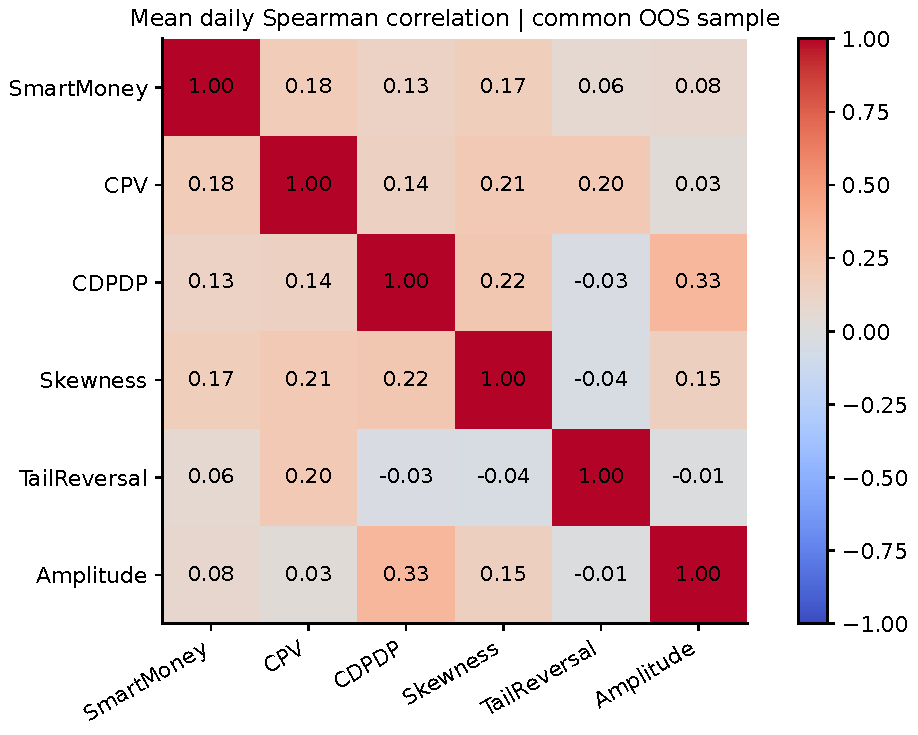
\includegraphics[width=0.65\linewidth,height=0.32\textheight,keepaspectratio]{correlation.pdf}
\caption{共同样本的六因子截面秩相关性}\label{fig:corr}
\end{figure}

XGBoost采用梯度提升树合成六个中性化因子\cite{chen}。每个N日期限单独训练，目标为
\begin{equation}
y^{(N)}_{i,T}=R^{(N)}_{i,T}-\frac{1}{|\mathcal U_T^*|}\sum_{j\in\mathcal U_T^*}R^{(N)}_{j,T},
\end{equation}
其中$\mathcal U_T^*$为历史训练截面中具有有效标签的股票集合。减去截面共同常数不会改变当天IC和RankIC。
预测股票池只由当时六个输入是否齐全决定，不按未来标签是否存在过滤。

每月首个交易日前训练一次，信号日期取最近12个月，且标签退出日必须严格早于该月首个交易日。
由此不同期限自动留下不同长度的标签实现间隔，不能统一仅留两天。
每个训练日期的总样本权重相同；固定100棵树、深度5、学习率0.05、随机种子42、hist算法，
不使用测试期调参或早停。2017年2月至2018年12月共23个月，每种期限23个模型，总计\ModelsCount 个模型。
\begin{table}[H]\centering\small
\caption{逐月训练范围核验}
\begin{tabular}{lrrrr}\toprule
期限 & 模型数 & 训练信号日数范围 & 训练股票日数范围 & 最晚标签退出日\\\midrule
周频 & 23 & 234--242 & 49,876--60,287 & 2018-11-30 \\
双周频 & 23 & 229--237 & 48,739--58,886 & 2018-11-30 \\
月频 & 23 & 219--227 & 46,196--56,489 & 2018-11-30 \\
\bottomrule
\end{tabular}\end{table}

\clearpage
\subsection{共同样本下的多频率绩效比较}
所有案例使用相同的\ComparisonStart 至\ComparisonEnd 信号区间、六因子完整股票样本、
调仓起点、费用和总敞口。测试期日均约\CommonMeanStocks 只股票，五分组每组约占20\%，不采用Top50。
统计量来自\ReturnDays 个每日费后收益；周、双周、月分别指每5、10、20个交易日，而非自然周末或月末。

\begin{table}[H]\centering\small
\caption{单因子与XGBoost的共同样本理论多空绩效}
\setlength{\tabcolsep}{4pt}\renewcommand{\arraystretch}{1.22}
\begin{tabular}{llrrrrrr}\toprule
频率 & 因子 & 原始IC & 原始RankIC & 年化收益 & Sharpe & 最大回撤 & 日均换手\\\midrule
周频 & SmartMoney & -0.038 & -0.036 & 0.37\% & 0.11 & -4.98\% & 21.14\% \\
 & CPV & -0.041 & -0.045 & 5.52\% & 1.48 & -2.34\% & 15.86\% \\
 & CDPDP & -0.030 & -0.042 & 4.43\% & 1.12 & -3.41\% & 12.98\% \\
 & Skewness & -0.031 & -0.039 & 2.96\% & 0.76 & -5.65\% & 15.01\% \\
 & TailReversal & -0.027 & -0.019 & -1.07\% & -0.23 & -7.72\% & 15.02\% \\
 & Amplitude & -0.018 & -0.039 & -0.36\% & -0.03 & -5.78\% & 9.94\% \\
\rowcolor{blue!8}
 & XGBoost & 0.041 & 0.048 & 4.49\% & 1.11 & -7.25\% & 21.43\% \\
\midrule
双周频 & SmartMoney & -0.035 & -0.035 & 0.32\% & 0.10 & -5.57\% & 14.82\% \\
 & CPV & -0.053 & -0.054 & 4.73\% & 1.24 & -2.16\% & 11.43\% \\
 & CDPDP & -0.037 & -0.050 & 3.60\% & 0.93 & -3.36\% & 9.34\% \\
 & Skewness & -0.037 & -0.045 & 2.16\% & 0.56 & -6.20\% & 10.68\% \\
 & TailReversal & -0.033 & -0.022 & -0.13\% & -0.01 & -6.16\% & 10.80\% \\
 & Amplitude & -0.017 & -0.038 & -0.63\% & -0.08 & -5.21\% & 7.87\% \\
\rowcolor{blue!8}
 & XGBoost & 0.041 & 0.045 & 2.08\% & 0.55 & -4.20\% & 12.70\% \\
\midrule
月频 & SmartMoney & -0.031 & -0.031 & 1.07\% & 0.31 & -3.84\% & 7.93\% \\
 & CPV & -0.068 & -0.074 & 7.14\% & 1.79 & -3.14\% & 7.88\% \\
 & CDPDP & -0.057 & -0.067 & 6.10\% & 1.55 & -2.81\% & 6.53\% \\
 & Skewness & -0.046 & -0.048 & 2.12\% & 0.54 & -8.56\% & 7.47\% \\
 & TailReversal & -0.031 & -0.032 & 0.84\% & 0.22 & -4.40\% & 7.56\% \\
 & Amplitude & -0.034 & -0.042 & 1.91\% & 0.38 & -3.62\% & 5.88\% \\
\rowcolor{blue!8}
 & XGBoost & 0.054 & 0.042 & 2.94\% & 0.80 & -3.59\% & 7.66\% \\
\midrule
\bottomrule
\end{tabular}\end{table}

表中换手为每日实际成交额除以当日交易前净资产后取均值，包含初始建仓及末日平仓，
不再称为“月均换手”。多空名义目标各50\%，不等同于原报告的100\%多头减100\%空头。
本表与旧数值的变化同时包含价格、交易、费用、样本与敞口调整，不能将差异归因于某一个修复。

XGBoost三种期限的IC均为正，但本次没有全面超越CPV：月频CPV年化\CPVMonthReturn、Sharpe\CPVMonthSharpe，
高于月频模型的\ModelMonthReturn、\ModelMonthSharpe；双周频CPV年化\CPVBiweekReturn，
也高于模型\ModelBiweekReturn。不能依据输入低相关就推断机器学习必然带来组合优势。

\clearpage
\subsection{多头分层、交易约束与估值诊断}
\begin{table}[H]\centering\small
\caption{共同样本双周频：五个多头组的费后年化收益及多头组回撤}
\begin{tabular}{lrrrrrr}\toprule
因子 & 第1组 & 第2组 & 第3组 & 第4组 & 第5组 & 第5组回撤\\\midrule
SmartMoney & -29.28\% & -21.28\% & -21.85\% & -19.60\% & -19.19\% & -41.57\% \\
CPV & -28.33\% & -27.24\% & -20.50\% & -17.19\% & -14.02\% & -38.71\% \\
CDPDP & -28.62\% & -22.64\% & -21.97\% & -15.25\% & -16.64\% & -35.52\% \\
Skewness & -27.97\% & -20.44\% & -22.42\% & -18.65\% & -17.71\% & -39.96\% \\
TailReversal & -28.00\% & -18.88\% & -19.74\% & -19.65\% & -21.04\% & -45.19\% \\
Amplitude & -23.34\% & -20.51\% & -20.90\% & -20.82\% & -18.21\% & -39.58\% \\
XGBoost & -28.85\% & -24.36\% & -17.95\% & -19.83\% & -16.96\% & -38.88\% \\
\bottomrule
\end{tabular}\end{table}
第5组为看好端；对于模型是高预测值，对于单因子是低原始因子值。
各多头组普遍亏损，理论多空的正收益主要体现不同股票之间的相对差异，而不是多头组合在该市场阶段获得绝对正收益。
分层也并非严格单调，例如XGBoost第3组与第4组顺序发生反转，应避免将分组图描述为完美排序。

\begin{table}[H]\centering\small
\caption{双周频理论多空：样本覆盖与执行、估值诊断}
\setlength{\tabcolsep}{4pt}
\begin{tabular}{lrrrrrr}\toprule
因子 & 日均信号股数 & IC覆盖率 & IC期数 & 缺行情股日 & 末日持仓数 & 最大绝对净敞口\\\midrule
SmartMoney & 218.4 & 98.82\% & 46 & 0 & 1 & 7.56\% \\
CPV & 218.4 & 98.82\% & 46 & 1 & 1 & 7.76\% \\
CDPDP & 218.4 & 98.82\% & 46 & 0 & 0 & 6.41\% \\
Skewness & 218.4 & 98.82\% & 46 & 0 & 0 & 5.43\% \\
TailReversal & 218.4 & 98.82\% & 46 & 0 & 1 & 5.58\% \\
Amplitude & 218.4 & 98.82\% & 46 & 0 & 0 & 4.83\% \\
XGBoost & 218.4 & 98.82\% & 46 & 0 & 0 & 8.70\% \\
\bottomrule
\end{tabular}\end{table}
缺行情股日统计持仓存在而报价状态未知的次数，已知停牌另按规则保留估值。
共同样本全部126条组合账本中，\OOSStaleSeries 条出现未知行情估值，\OOSUnclosedSeries 条期末仍有持仓；
21个理论多空案例中分别有\OOSLSStaleCases 个和\OOSLSUnclosedCases 个。
这些记录不能被删掉后重新选股，涉及的收益也不能当作已清算现金收益。
\texttt{HasStaleValuations}与\texttt{FullyLiquidated}在原始汇总表中保留。

目标多空各50\%不保证每天净敞口为0：价格变化、受阻卖出与现金留存会使实际头寸偏离目标。
表中已报告最大绝对净敞口，因此理论多空也不能直接解释为完全消除了市场风险的Alpha。

\clearpage
\subsection{模型年度表现与输入重要性}
表\ref{tab:year}按日收益复利分年统计，2017年只包括2月6日至年末，2018年为本地交易日历内完整年份。
年度收益没有再次年化。XGBoost双周频2017年为正、2018年为负，说明全期正年化不能掩盖分阶段表现差异。
\begin{table}[H]\centering\small
\caption{双周频理论多空的分年收益}\label{tab:year}
\begin{tabular}{lrrr}\toprule
因子 & 2017年（部分年度） & 2018年 & 全样本年化\\\midrule
SmartMoney & 5.42\% & -4.57\% & 0.32\% \\
CPV & 3.88\% & 4.96\% & 4.73\% \\
CDPDP & 4.93\% & 1.83\% & 3.60\% \\
Skewness & 7.55\% & -3.22\% & 2.16\% \\
TailReversal & 3.16\% & -3.29\% & -0.13\% \\
Amplitude & -0.90\% & -0.28\% & -0.63\% \\
XGBoost & 5.16\% & -1.16\% & 2.08\% \\
\bottomrule
\end{tabular}\end{table}
\begin{figure}[H]\centering
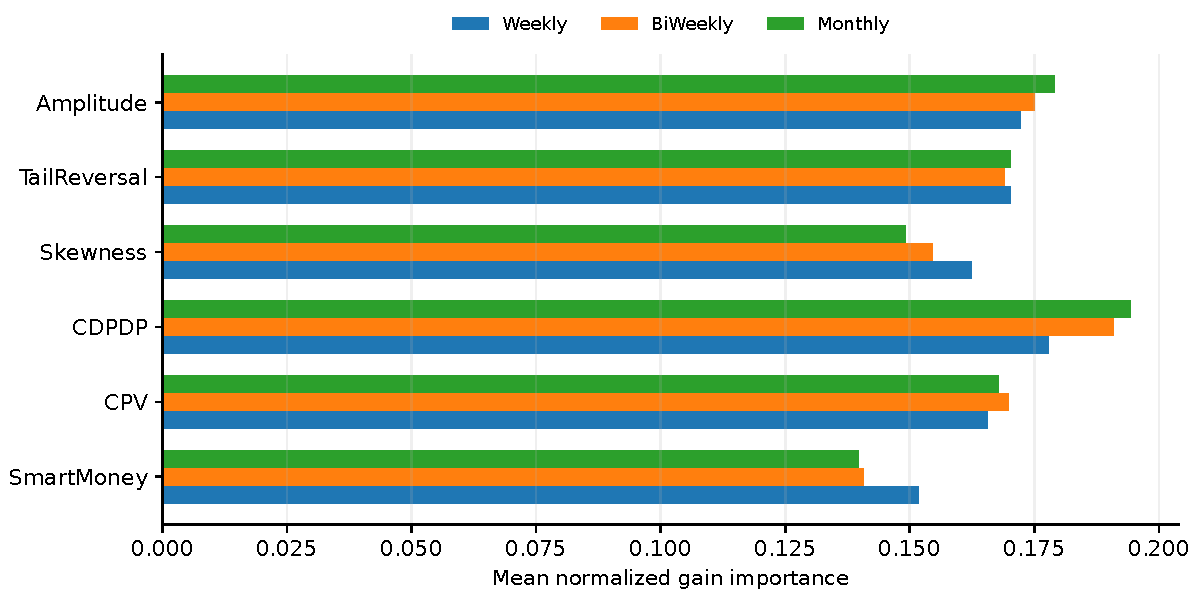
\includegraphics[width=0.90\linewidth,height=0.31\textheight,keepaspectratio]{importance.pdf}
\caption{按预测期限分别汇总的逐月模型平均归一化增益重要性}
\end{figure}
重要性来自每个月独立拟合的树模型，反映特征参与分裂所带来的相对增益；
它不表明作用方向，更不构成因果解释。重要性较高也不意味着单因子一定具有最高的费后收益，
因为模型可以依赖条件关系，而且交易结果还受换手和执行约束影响。
三个期限分别建模，不能将某个期限的分数直接当作其他期限标签的预测结果。

\clearpage
\subsection{双周频分层净值与理论多空曲线}
\navfigure{HF_SmartMoney_BiWeekly}{SmartMoney因子的共同样本双周频回测}
\vfill
\navfigure{HF_Raw_CPV_Mean_BiWeekly}{CPV因子的共同样本双周频回测}
\clearpage

\navfigure{HF_CDPDP_BiWeekly}{CDPDP因子的共同样本双周频回测}
\vfill
\navfigure{HF_Skewness_BiWeekly}{Skewness因子的共同样本双周频回测}
\clearpage

\navfigure{HF_Tail_Reversal_BiWeekly}{TailReversal因子的共同样本双周频回测}
\vfill
\navfigure{HF_Amplitude_BiWeekly}{Amplitude因子的共同样本双周频回测}

\clearpage
\subsection{XGBoost分层与不同期限净值}
\navfigure{Pred_Score_BiWeekly}{XGBoost共同样本双周频分层与理论多空净值}
\vfill
\begin{figure}[H]\centering
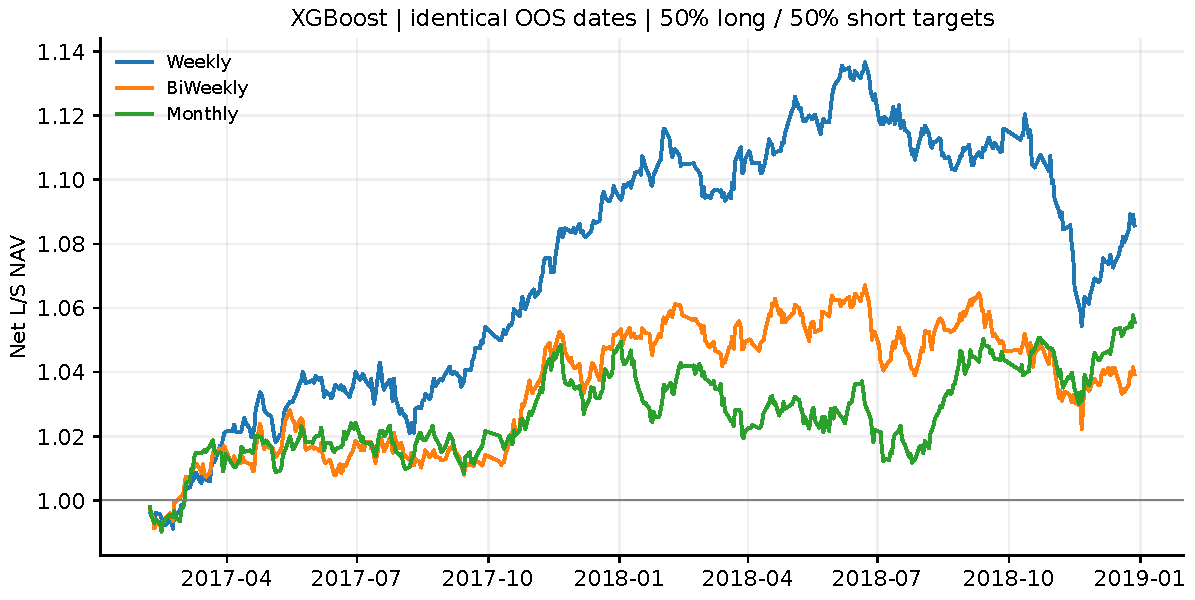
\includegraphics[width=0.95\linewidth,height=0.36\textheight,keepaspectratio]{model_horizons.pdf}
\caption{XGBoost三个期限的理论多空净值，均由各自实际持仓日账本计算}
\end{figure}

\clearpage
\section{因子思考与改进}
\subsection{模型排序能力与交易收益并非同一指标}
模型周频原始RankIC为\ModelWeekRank，月频为\ModelMonthRank，说明分数具有一定的截面排序信息；
但IC覆盖完整截面，而组合只持有两端分组，且需承担费用、持仓漂移和不可成交影响。
因此月频IC较高并不要求月频费后收益一定超过周频，也不能用某个月的IC替代同期限策略回测。
后续应分别检验极端分数组的收益稳定性、不同市场阶段的排序一致性，以及更低换手的目标权重设计。

\subsection{因子互补性不自动转化为模型优势}
相同样本下，CPV三个期限的理论多空年化均高于XGBoost，说明本次非线性合成没有稳定超越最好的输入。
可能原因包括有限历史、标签噪声、树模型在市场阶段变化时不稳定，以及输入已经中性化后可利用的非线性关系较弱。
这些是待检验的解释，不是已经识别的原因。若继续调参，应在训练历史内部设置按时间排列且按标签退出日隔离的验证段，
并保留新的最终测试期；不宜围绕本文测试结果反复优化再报告同一段收益。

\subsection{可交易性与数据完整性仍是研究边界}
本次4.9\%开盘跳空过滤仅为日行情条件下的成交代理；实际涨跌停价、排队与借券供应需要额外数据。
连续价格单位相当于除权权益即时再投资，未模拟分红到账、整手和冲击成本。
少量未知尾部行情仍使用最近估值，退市清算与实际回收价值没有由现有数据确定。
下一步应优先补充这些数据，再做借券费、滑点和成交阈值敏感性分析，而不是将当前理论多空收益直接当作可执行收益。

\section{结论}
本文完成了2016至2018年六个高频因子的完整检验，并在共同样本外区间训练\ModelsCount 个XGBoost模型。
在统一价格、期限、交易日历和费用后，模型周、双周、月频理论多空年化分别为
\ModelWeekReturn、\ModelBiweekReturn、\ModelMonthReturn；周频Sharpe为\ModelWeekSharpe，最大回撤为\ModelWeekDD。
模型具有正向排序信息，但单因子CPV在本次三个期限下均提供更高的理论多空年化收益。

本研究支持“高频因子含有可研究的相对选股信息”，不支持“非线性合成必然提升收益”或“回测已证明可直接实盘获利”。
多头绝对亏损、实际净敞口偏离、尾部估值和借券假设都应与多空指标同时报告。
原报告的旧模型收益和回撤不再作为本次结果引用；后续研究应在新的时间样本及更完整的交易数据上继续验证。

\clearpage
\section{代码输出与可复现性}
本次从独立输出目录重新执行完整流程，包含731个分钟文件、18个完整时期单因子案例，
以及共同样本下21个单因子或模型案例。共核对\AllSeries 条组合账本、\TradesCount 笔成交，
现金流、费用、净值与汇总风险指标一致。26项单元测试通过，训练标签退出日和三种模型预测样本一致性均已检查。

\begin{Verbatim}[fontsize=\small,frame=single,breaklines=true]
python code2_new.py --with-xgboost \
  --output-dir results_code2_new_report
python -m unittest discover -s tests -p 'test_code2*.py' -v
python report_new/build_report.py
\end{Verbatim}

\begin{table}[H]\centering\small
\caption{XGBoost本次实际输出摘要（共同样本理论多空）}
\begin{tabular}{lrrrr}\toprule
频率 & IC & RankIC & 年化收益 & Sharpe\\\midrule
周频 & \ModelWeekIC & \ModelWeekRank & \ModelWeekReturn & \ModelWeekSharpe\\
双周频 & \ModelBiweekIC & \ModelBiweekRank & \ModelBiweekReturn & \ModelBiweekSharpe\\
月频 & \ModelMonthIC & \ModelMonthRank & \ModelMonthReturn & \ModelMonthSharpe\\\bottomrule
\end{tabular}\end{table}

完整产物保存在\path{results_code2_new_report/}：根目录为全时期单因子结果，
\path{xgboost/}保存逐月模型、预测、训练范围与重要性，\path{comparison/}保存共同样本全部21个案例。
每个案例含\texttt{signal\_groups.parquet}、\texttt{ic.csv}、\texttt{daily\_ledger.csv}、
\texttt{trades.parquet}与\texttt{nav.png}。本文表格、图和数值由这些文件自动生成，未手工改写绩效。

\subsection*{完整源代码附件}
报告配套目录\path{source/}包含主流程、XGBoost模块和测试文件；PDF同时嵌入两个完整源码附件。
支持附件面板的阅读器可直接提取：
\begin{itemize}
\item 主流程：\attachfile[icon=Paperclip,mimetype=text/plain]{source/code2_new.py}\quad\texttt{code2\_new.py}。
\item 模型模块：\attachfile[icon=Paperclip,mimetype=text/plain]{source/code2_xgboost.py}\quad\texttt{code2\_xgboost.py}。
\end{itemize}
主文件与模型文件应放在同一目录。原\texttt{code2.py}、原报告及旧图片保持原样。
逐月训练日志、运行参数、源码摘要和对账记录随报告源文件一起保存，便于核查结果对应的实现版本。

\clearpage
\appendix
\section{全时期单因子结果与参考资料}
下表恢复较长样本的单因子观察区间：信号2016-01-29至2018-12-28，711个日收益。
股票样本为各单因子自身有效样本，没有套用共同六因子完整条件，因此不能将其数值直接与主文XGBoost表比较。
原始完整流程生成的18幅净值图均保存在对应结果目录，附录B另展示共同测试样本的周、月频图。
\begin{table}[H]\centering\small
\caption{全时期六因子理论多空绩效（独立有效样本）}
\begin{tabular}{llrrrrr}\toprule
频率 & 因子 & 原始IC & 原始RankIC & 年化收益 & Sharpe & 最大回撤\\\midrule
周频 & SmartMoney & -0.039 & -0.045 & 2.21\% & 0.77 & -2.40\% \\
 & CPV & -0.037 & -0.049 & 4.14\% & 1.65 & -1.51\% \\
 & CDPDP & -0.040 & -0.050 & 8.47\% & 2.05 & -2.84\% \\
 & Skewness & -0.039 & -0.052 & 4.83\% & 1.78 & -1.81\% \\
 & TailReversal & -0.028 & -0.026 & 1.66\% & 0.54 & -4.45\% \\
 & Amplitude & -0.025 & -0.047 & 2.79\% & 0.57 & -6.27\% \\
\midrule
双周频 & SmartMoney & -0.043 & -0.052 & 2.25\% & 0.84 & -2.74\% \\
 & CPV & -0.044 & -0.055 & 4.03\% & 1.61 & -1.94\% \\
 & CDPDP & -0.053 & -0.064 & 8.07\% & 1.95 & -3.47\% \\
 & Skewness & -0.050 & -0.059 & 4.74\% & 1.78 & -2.10\% \\
 & TailReversal & -0.029 & -0.024 & 1.51\% & 0.51 & -4.52\% \\
 & Amplitude & -0.038 & -0.059 & 3.08\% & 0.64 & -4.84\% \\
\midrule
月频 & SmartMoney & -0.037 & -0.046 & 2.82\% & 1.09 & -2.27\% \\
 & CPV & -0.049 & -0.058 & 3.45\% & 1.36 & -3.30\% \\
 & CDPDP & -0.069 & -0.084 & 7.07\% & 1.67 & -3.49\% \\
 & Skewness & -0.059 & -0.071 & 4.20\% & 1.62 & -3.30\% \\
 & TailReversal & -0.027 & -0.024 & 1.04\% & 0.36 & -5.31\% \\
 & Amplitude & -0.048 & -0.072 & 4.35\% & 0.91 & -5.40\% \\
\midrule
\bottomrule
\end{tabular}\end{table}

\begingroup\small
\begin{thebibliography}{9}
\bibitem{course} 《量化投资》课程作业说明与随附本地行情、交易日历、行业及市值数据字典。
\bibitem{chen} Chen T., Guestrin C. XGBoost: A Scalable Tree Boosting System. 2016.
\url{https://arxiv.org/abs/1603.02754}.
\bibitem{sharpe} Sharpe W. F. The Sharpe Ratio. The Journal of Portfolio Management, Fall 1994.
\url{https://web.stanford.edu/~wfsharpe/art/sr/SR.htm}.
\bibitem{local} 本次运行产物：\texttt{run\_config.json}、\texttt{comparison\_config.json}、
\texttt{training\_log.csv}、\texttt{validation.json}与随附完整源代码，\ReportDate。
\end{thebibliography}
\endgroup

\clearpage
\section{周频与月频完整净值图}
\navfigure{HF_SmartMoney_Weekly}{SmartMoney的共同样本周频回测}
\vfill
\navfigure{HF_SmartMoney_Monthly}{SmartMoney的共同样本月频回测}
\clearpage

\navfigure{HF_Raw_CPV_Mean_Weekly}{CPV的共同样本周频回测}
\vfill
\navfigure{HF_Raw_CPV_Mean_Monthly}{CPV的共同样本月频回测}
\clearpage

\navfigure{HF_CDPDP_Weekly}{CDPDP的共同样本周频回测}
\vfill
\navfigure{HF_CDPDP_Monthly}{CDPDP的共同样本月频回测}
\clearpage

\navfigure{HF_Skewness_Weekly}{Skewness的共同样本周频回测}
\vfill
\navfigure{HF_Skewness_Monthly}{Skewness的共同样本月频回测}
\clearpage

\navfigure{HF_Tail_Reversal_Weekly}{TailReversal的共同样本周频回测}
\vfill
\navfigure{HF_Tail_Reversal_Monthly}{TailReversal的共同样本月频回测}
\clearpage

\navfigure{HF_Amplitude_Weekly}{Amplitude的共同样本周频回测}
\vfill
\navfigure{HF_Amplitude_Monthly}{Amplitude的共同样本月频回测}
\clearpage

\navfigure{Pred_Score_Weekly}{XGBoost的共同样本周频回测}
\vfill
\navfigure{Pred_Score_Monthly}{XGBoost的共同样本月频回测}
\end{document}
